

\section{Paper Summary}
This section gives a summary of the method presented in the paper, outlined in Figure \ref{fig:pipeline},
with an emphasis on explaining concepts that did not receive a lot of attention in the paper.

\begin{figure*}
    \centering
    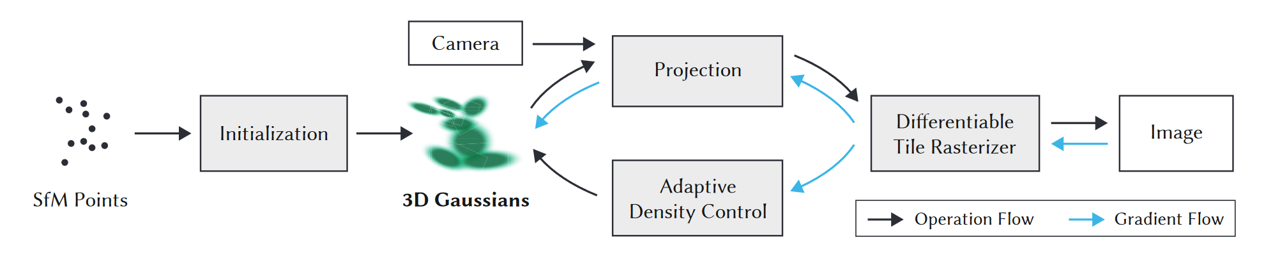
\includegraphics[width=\textwidth]{images/pipeline.png}
    \caption{The Gaussian splatting pipeline presented in the paper \cite[Fig. 2]{kerbl3DGaussianSplatting2023}.}
    \label{fig:pipeline}
\end{figure*}


\subsection{Representation}
The core idea of the paper is to represent the scene as a set of Gaussians.
Each Gaussian is defined by its position $\bm{\mu}$, its covariance matrix $\bm{\Sigma}$, its opacity $\alpha$ and its spherical harmonic coefficients $\bm{c}$ used to give it a view-dependent color, further discussed in Section \ref{sec:spherical_harmonics}.
The covariance is defined as
\begin{align}
    \bm{\Sigma} = \bm{R} \bm{S} \bm{S}^T \bm{R}^T,
\end{align}
where $\bm{R}$ is a rotation matrix stored as a quaternion $\bm{q}$ and $\bm{S}$ is a diagonal matrix containing the standard deviation of the Gaussian along each axis, stored as a vector $\bm{s}$.
To ensure that the covariance is positive definite, the values of $\bm{s}$ are passed through a sigmoid activation function, and quaternion $\bm{q}$ is normalized to ensure a proper rotation matrix.
In total, each Gaussian has 59 parameters, 3 for the position, 3 for the scale, 4 for the quaternion 1 for alpha and 48 for the spherical harmonic coefficients.


\subsection{Projection}
The first step of the rendering pipeline, shown in Figure \ref{fig:pipeline}, is to project the Gaussians onto the image plane.
First, the Gaussians are transformed into the camera frame using a linear view transformation $\bm{W}$.
Then the Gaussians are projected onto the image plane using a pinhole projection.
This transformation is visualized by comparing Figure \ref{fig:proj_2a} and Figure \ref{fig:proj_2b}.


\begin{figure}[t]
    \centering
    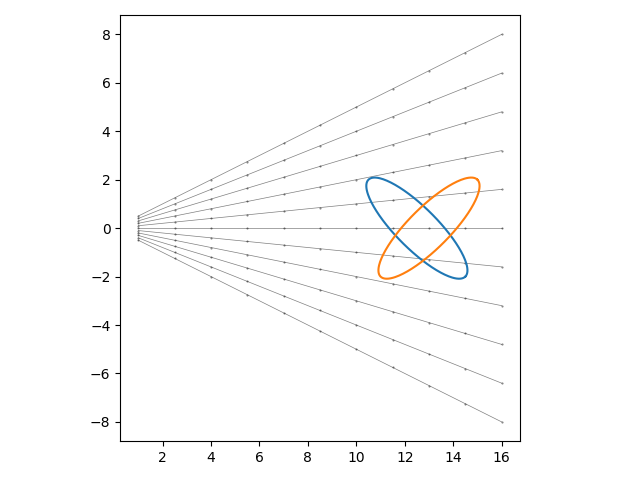
\includegraphics[width=\linewidth]{images/proja.png}
    \caption{Covariance ellipses of two Gaussians in the camera frame viewed from the side, with visualization of pixel rays.}
    \label{fig:proj_2a}
\end{figure}


Two key steps are performed to speed up the projection process.
First, instead of accurately projecting the Gaussians onto the image plane, a linear approximation is used where the center point is projected properly, but the covariance is updated given the following linear approximation,
\begin{align}
    \bm{\Sigma'} & = \bm{J} \bm{W} \bm{\Sigma} \bm{W}^T \bm{J}^T \label{eq:linear_approx}
\end{align}
where $\bm{J}$ is the Jacobian of the projection function.
The result of this approximation is visualized as the two dotted ellipses in Figure \ref{fig:proj_2b}.

A second significant speedup step is to remove the depth component of the projected Gaussians, resulting in a 2D Gaussian with position $\bm{\mu}''$ and covariance $\bm{\Sigma}''$, visualized as a line in Figure \ref{fig:proj_2b}.
The key benefit of this is that the depth ordering of the Gaussians is identical for each pixel.
This does however introduce a significant issue, where small changes in view direction can decide which Gaussian is in front of another Gaussian, resulting in strong popping artifacts, which the paper acknowledges \cite[Sec 7.4]{kerbl3DGaussianSplatting2023}.

\begin{figure}[htb]
    \centering
    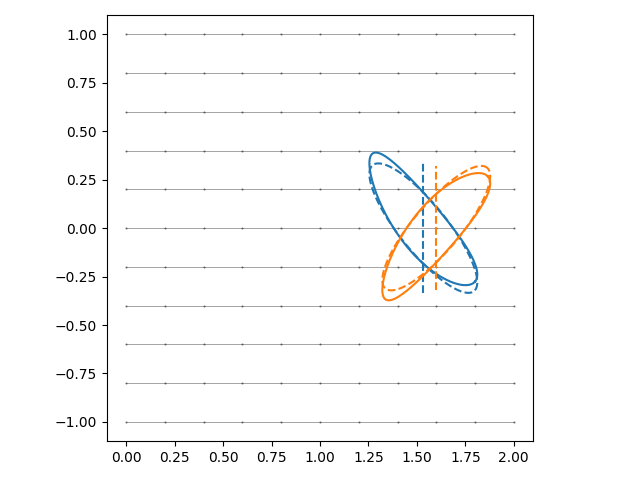
\includegraphics[width=\linewidth]{images/projb.png}
    \caption{The camera projection of Figure \ref{fig:proj_2a}. The dotted lines are the linear approximation of the Gaussians given Equation \ref{eq:linear_approx} and the vertical line is the simplification from removing the depth component}.
    \label{fig:proj_2b}
\end{figure}

\begin{align}
    G(\bm{x}) & =  \label{eq:gaussian_density_function}
\end{align}
where $\bm{x}$.


\subsection{Rasterization Pipeline}
As shown in Figure \ref{fig:pipeline}, the rendering pipeline consists of two phases, a projection phase and a rasterization phase.

\label{sec:rasterization}
\begin{figure}
    \centering
    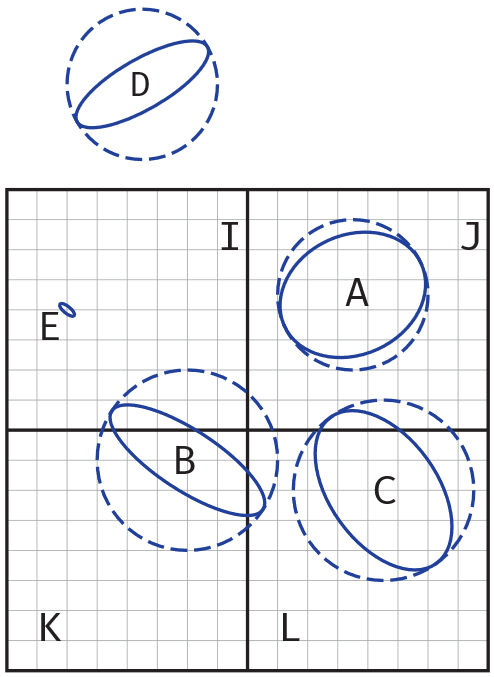
\includegraphics[width=0.6\linewidth]{images/rendering.png}
    \caption{Visualization of how Gaussian splats are rendered using multiple independent blocks.}
\end{figure}

After dubplicating, sorting and separating the projected gaussians, each pixel is rendered independently following a standard alpha blending approach with the following blending function,

\begin{align}
    C   & = \sum_{i \in N} c_i a_i \prod_{j=1}^{i-1} (1-a_j)                                           \\
    a_i & = \alpha_i e^{-\frac{1}{2}(\bm{x}-\bm{\mu}''_i)^T\bm{\Sigma''}_i^{-1} (\bm{x}-\bm{\mu}''_i)}
    \label{eq:alpha_blending}
\end{align}


where $C$ is the resulting color, $c_i$ is the color of the $i$'th Gaussian calculated from the view direction and its spherical harmonic coefficients, $a_i$ is the opacity of the $i$'th Gaussian which is the product of its overall opacity $\alpha_i$ and the evaluation of the Gaussian density function at the pixel location of the 2D projected Gaussian given in Equation \ref{eq:gaussian_density_function}.

\subsection{Densification}
\begin{figure}
    \centering
    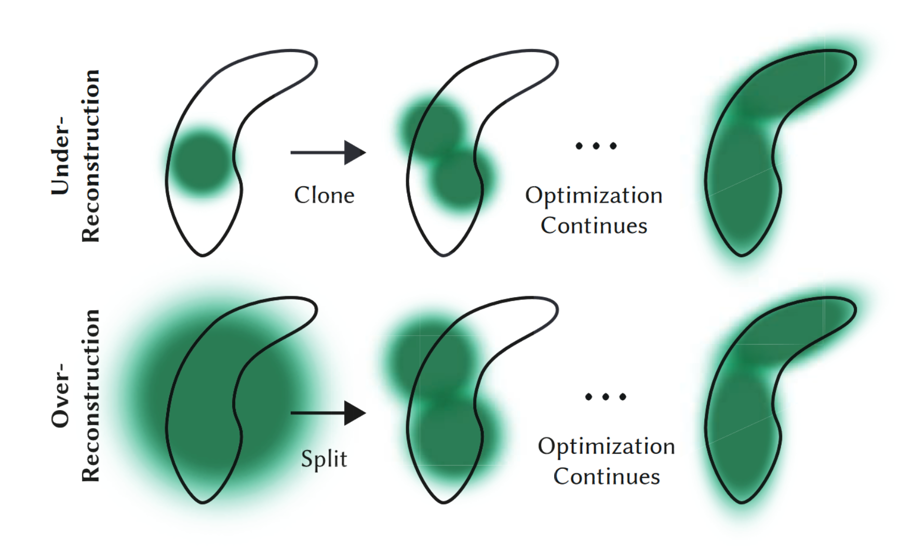
\includegraphics[width=\linewidth]{images/densification.png}
    \caption{The adaptive Gaussian densification scheme presented in the paper \cite[Fig. 4]{kerbl3DGaussianSplatting2023}.}
\end{figure}
